Before we talk about the compiler driver in Clang, it is necessary to highlight the fact that compiling a piece of code is never a single task (and not a simple one, either). In school, we were taught that a compiler consists of a lexer, a parser, sometimes came with an optimizer, and ended with an assembly code printer. While you still can see these stages in real-world compilers, they give you nothing but textual assembly code rather than an executable or library, as we would normally expect. Furthermore, this naïve compiler only provides limited flexibility – it can't be ported to any other operating systems or platforms.

To make this toy compiler more realistic and usable, many other plumber tools need to be put together, along with the core compiler: an assembler to transform assembly code into (binary format) object file, a linker to put multiple object files into an executable or library, and many other routines to resolve platform-specific configurations, such as data width, default header file paths, or Application Binary Interfaces (ABIs). Only with help from these plumbers can we use a compiler by just typing a few words:

\begin{tcblisting}{commandshell={}}
$ clang hello_world.c -o hello_world
\end{tcblisting}

A compiler driver is software that organizes these plumber jobs. Despite having multiple different tasks to do during the compilation, we will only focus on two of the most important ones in this chapter – handling compiler flags and invoking the right tools on different platforms – which is what toolchains are designed for.

The following diagram shows the interactions between the driver, the toolchains, and the rest of the compiler:

\hspace*{\fill} \\ %插入空行
\begin{center}
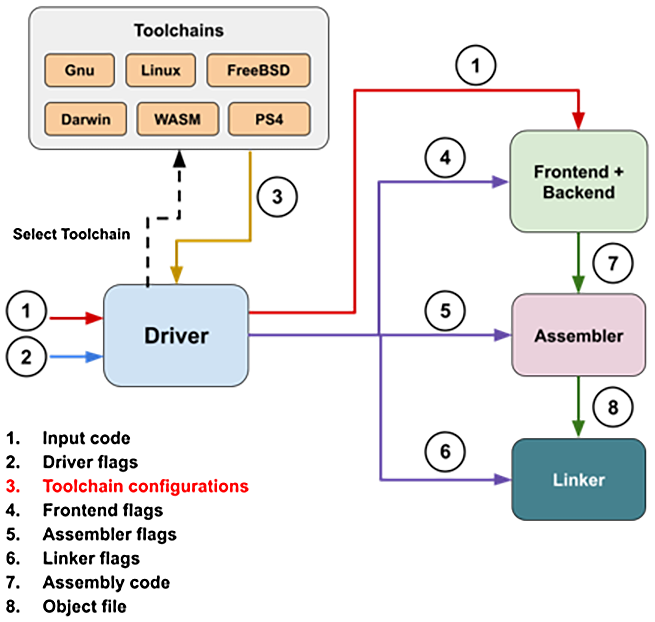
\includegraphics[width=0.9\textwidth]{content/2/chapter8/images/1.png}\\
Figure 8.1 – Typical workflow of Clang's driver, toolchains, and the rest of the compiler
\end{center}

As shown in the preceding diagram, Clang's driver acts as a dispatcher and distributes flags and workloads to each of the compilation phases, namely the frontend/backend, the assembler, and the linker. To give you a more concrete idea of what the flags for each of these phases look like, recall the -\#\#\# compiler option we introduced at the beginning of this chapter. The (massive amount of) content that's printed by that option is the flags for the frontend (4 in the preceding screenshot). For example, among those frontend flags, -internal-isystem carries the information about the system header path, including the path where the C/C++ standard library header files are stored. It is obvious that Clang's frontend needs to know where the standard library headers are stored, but as per your past experiences of using clang (or gcc), you rarely need to tell them where those headers are explicitly – the driver will do that for you. The same logic applies to the linking phase as well. Linkers usually need more than just an object file to properly generate an executable or a library. For example, they need to know where the C/C++ standard library's library files (*.a or *.so on Unix/Linux systems) are. In that case, Clang's driver will provide that information to the linkers via linker flags.

Flags and workloads – or configurations, in short – that are provided to individual compiler phases are translated from two sources: driver flags (2 in the preceding diagram) and the selected toolchain (3 in the preceding diagram). Driver flags are those provided by users via the command-line interface – that is, the compiler flags– such as -c, -Wall, and -std=c++11. In the next section, Adding custom driver flags, we will show you some examples of how Clang translates driver flags into frontend flags or even assembler/linker flags.

On the other hand, a toolchain is an entity that describes how input code should be compiled on a specific platform. Different hardware architectures and operating systems (OS) – platforms, for short – have their own way to build, load, and run programs. Take macOS X and Linux, for example. Although they both have a Unix-like environment, when building a program, the system (standard) libraries for macOS X always reside in Apple's XCode IDE package, whereas Linux usually stores them in normal folders such as /usr/include and /usr/lib. Also, macOS X uses an executable format called Mach-O, which is different from Linux's ELF format. This greatly affects how compilers (Clang) build the code.

For Clang to compile code for various platforms, it uses toolchains (which are effectively represented by the ToolChain C++ class internally) to encapsulate platform-specific information and configurations. In the early stage of compilation, Clang's driver selects a correct toolchain based on the system currently running (called the host system) or the users' preference – you can use the -target= driver flag to ask Clang to build a program for a specific platform that is different from the host system, which is effectively doing cross-compiling. Then, the driver will gather some platform-specific configurations from the selected toolchain before combining it with the aforementioned driver options and dispatching them to individual compiler phases via command-line flags. Note that different platforms usually use different assemblers and linkers. For example, macOS X can only use ld64 and lld linkers for now, whereas Linux can use ld (BFD linker), ld.gold, and lld as linkers. Therefore, a toolchain should also specify what assembler and linker to use. In the last section of this chapter, Adding a custom toolchain, we will go through an example project to learn how Clang's toolchains work. Let's start our journey by learning how driver flags work in Clang.






























